\chapter{Planificación}\label{chap:planif}
La planificación de un proyecto es fundamental para su correcto funcionamiento y desarrollo,
dentro de los plazos y costes establecidos. En este apartado se detallan las tareas que se
llevarán a cabo en el proyecto, así como los recursos necesarios y los plazos de ejecución.

\section{Metodología}\label{sec:metodología}
\subsection{Scrum}\label{subsec:scrum}
Para la planificación del proyecto se ha escogido \textit{Scrum}, una metodología ``ágil'' que se
basa en la realización de iteraciones cortas y en la adaptación a los cambios. La metodología
\textit{Scrum} se estructura en \textit{sprints} (iteraciones cortas de una duración fija),
en las que se llevan a cabo una serie de tareas que se han planificado previamente.

El primer paso de la metodología \textit{Scrum} es la creación de un \textit{product backlog},
una lista ordenada de las tareas a realizar durante el desarrollo del producto, a partir de los
requisitos del sistema, que a su vez son una versión refinada de los requisitos iniciales del
proyecto. A partir de este \textit{product backlog} se planifican las tareas que se llevarán
a cabo en cada \textit{sprint}, de manera que sea posible cumplir con los objetivos del proyecto
en el tiempo establecido.

\subsection{Visualización de la planificación}\label{subsec:visual_planif}
Para la visualización de la planificación se ha utilizado la herramienta de gestión de proyectos
de \textit{GitHub}, que permite múltiples visualizaciones de tareas e \textit{issues} en tableros
separados.

\begin{itemize}
	\item Se utiliza un tablero de \textit{requisitos} al estilo \textit{Kanban} para visualizar
		los requisitos del proyecto y su estado, siguiendo con la metodología \textit{Scrum}.
	\item Se utiliza un \textit{roadmap} de tareas, donde se visualizan las tareas y los hitos
		del proyecto, así como su estado y sus fechas límite.
\end{itemize}

\begin{minipage}{\linewidth}
	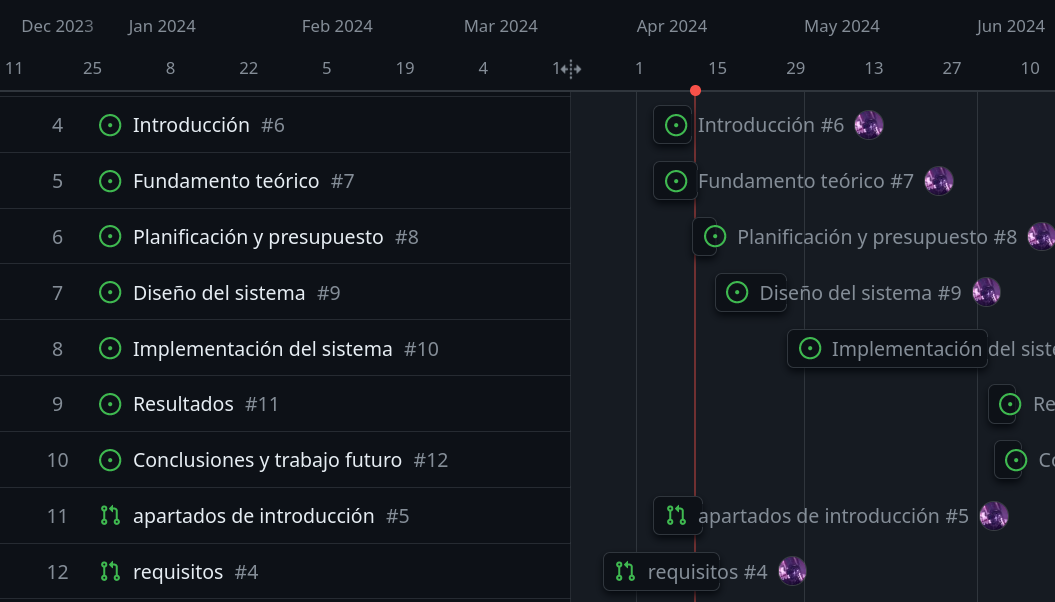
\includegraphics[width=0.95\textwidth]{roadmap.png}
	\captionof{figure}{Roadmap de tareas}
\end{minipage}

\subsection{Comunicación}\label{subsec:comunicación}
La comunicación con los tutores y con el equipo de desarrollo se considera fundamental para el
correcto desarrollo del proyecto. Puesto que el trabajo se desarrolla de manera presencial en
la oficina de la empresa, la comunicación con el equipo de desarrollo se realiza de manera
frecuente y directa, mientras que la comunicación con los tutores se realiza de manera remota
pero igual de frecuente, manteniendo el contacto mediante correo electrónico y Teams para
pedir revisiones e informar sobre el estado del trabajo en todo momento.
\newpage{}
\section{Presupuesto}\label{sec:presupuesto}
